\paragraph{NQM Loss on Pretrained Model}
\label{experiments:02.2.1:Only_NQM_Pretrained}
As a first "naive" test to circumvent the problems in \autoref{experiments:01.1:Only_NQM}, before we developed the DiceBceNQM (\autoref{experiments:02.1:diceBce+NQM}), we have taken a pretrained models with the DiceBCE.

\begin{align}
    \ell(y_i, f_\theta(x_i))\ :=
      \begin{cases}
        \mathrm{DiceBCE} & \text{if epoch {\color{red}$\leq n$}}\\
        \mathrm{NQM} & \text{else}\\
      \end{cases}
\end{align}

Regardless of how long the model was pretrained, as soon as the loss was switched to the NQM the loss dropped enormously quickly towards zero, for the same reason, as for the NQM alone. The output looks the same as in \autoref{fig:exp.01.1:DiceBce_vs_NQM_only} (left).

%%% Alternating
Since it is only a little adjustment form there, we also checked, if this can already be prevented if we alternate between the NQM and DiceBCE. So the loss becomes:

\begin{align}
    \ell(y_i, f_\theta(x_i))\ :=
      \begin{cases}
        \mathrm{NQM} & \text{if epoch {\color{red} mod $x=0$}}\\
        \mathrm{DiceBce} & \text{else}\\
      \end{cases}
\end{align}

However, this attempt suffers from the same problem. For comparison, \autoref{fig:exp.02.1:alternating} shows that already after three epochs on the NQM, the output looks as bad as \autoref{experiments:01.1:Only_NQM} and moreover, already in the very first epoch no useful prediction is left anymore So, for larger $x$ this attempt only takes longer but still converges to the same state, while the epochs with the DiceBCE work in the opposite direction.

\begin{figure}[h!]
    \centering
    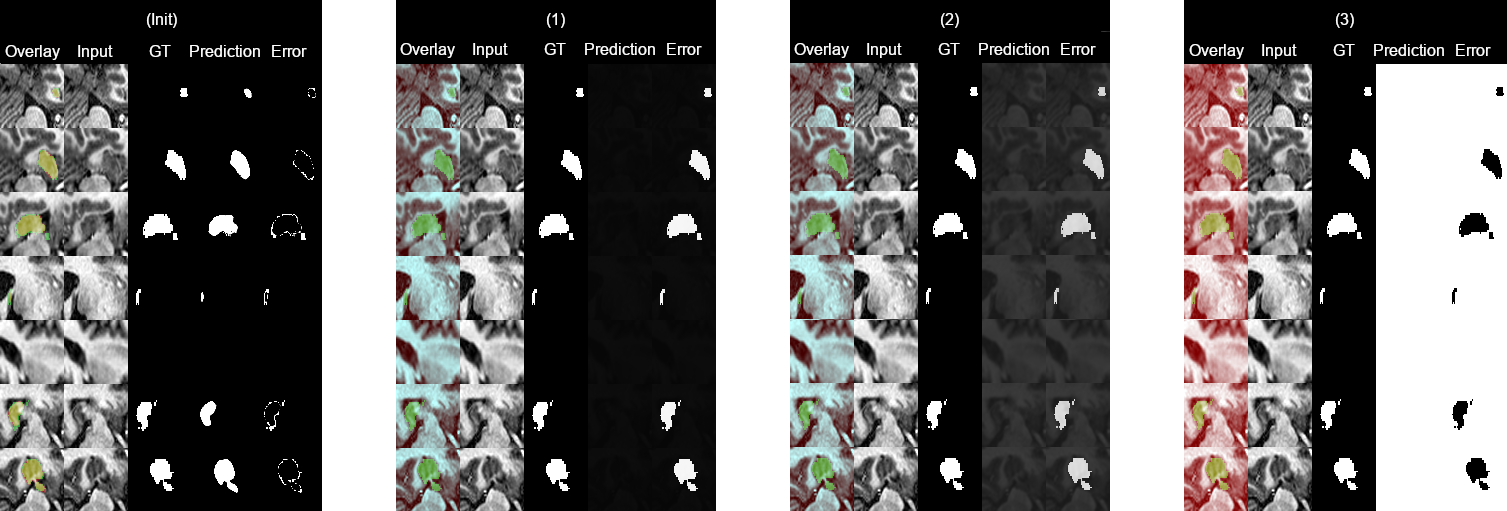
\includegraphics[width=\linewidth]{Graphics/Experiments/4.2.1_Alternating_3epochs_v3.png}
    \caption{Image samples volumes (inputs) with ground truth labels (GT), predictions, and errors. The overlay shows the input image with false positive (red), true positive (yellow), and  false negative (green). From left to right: The initial state, pretrained on DiceBCE (Init), the three very first epochs of training on the NQM.}
    \label{fig:exp.02.1:alternating}
\end{figure}